\section{Challenges}
\subsection{Client}
\subsubsection{Testing Clients}
The front-end is written in React and is composed of presentational components (components), stateful components (containers) and hooks. In separating presentational and stateful components from one another we wanted to ease testing. Although testing presentational components took place without a problem using Jest.js snapshots, render tests and some simple consistency tests, stateful containers were harder to test, since they required extensive mocking of React's hook and lifecycle events.

\subsubsection{Sensor Data Collection}
\paragraph{Browser Inconsistencies} \

\textit{from https://github.com/PSE-TECO-2020-TEAM1/client/issues/5\#issuecomment-817308653}

There are two main APIs on sensor access in browsers right now, namely the Sensors API, which is incorporated into the web standard and supported by 71.03\% of all users worldwide.

On the other hand there is the legacy DeviceMotionEvent API, which was an experimental technology designed before the aforementioned Sensors API was drafted. It is supported by 94.97\% of users worldwide (albeit with handicaps).

In this application, we are using the new standard Sensors API, which is only supported by Chrome and Chromium based browsers like Edge, Brave etc. for now. Apple refuses to implement the new API citing privacy concerns, there is no information on why Firefox doesn't implement it. Since on Apple platforms all browsers from all vendors use the Safari WebView, this new API doesn't work at all on Apple devices.

The DeviceMotionEvent API is unfortunately not suitable for use at all. All three different major browsers (Chrome, Safari and Firefox) have a different understanding of what coordinates they return and have no documentation of which units they return the data in.

We've tried to use a polyfill with the branch sensors-polyfill, but were getting totally different results with different browsers (and with firefox totally broken results. Because of this reason we've decided not to support Apple users at all.

\paragraph{Magnetometer} \
Originally we wanted to support Magnetometer sensor too, since it was (supposedly) supported by the browsers we were targeting (on caniuse.com).
\begin{center}
\end{center}

\begin{figure}[ht]
    \centering
    \fbox{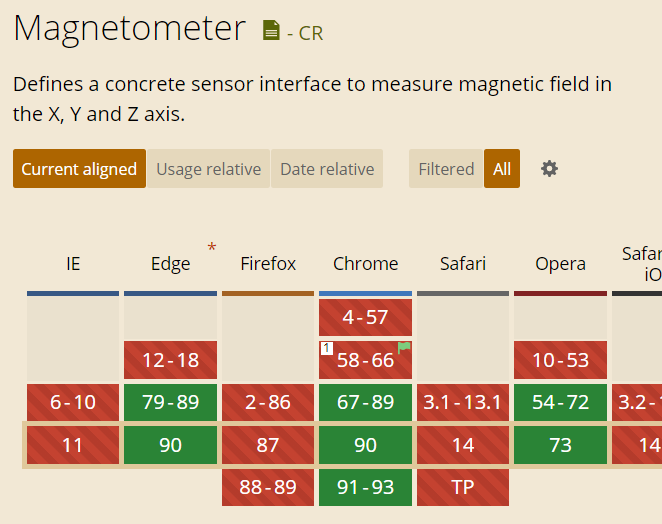
\includegraphics[width=\textwidth]{images/magneto1.png}}
    \caption{caniuse.com - Magnetometer}
\end{figure}



After implementing the sensor, however, we've noticed how no matter what we've tried, we weren't getting any data, and after more investigations we've discovered that the 'Magnetometer Sensor' and the 'Magnetometer Sensor API' are two different entities separate from each other, and dropped support for magnetometers.

\begin{figure}[ht]
    \centering
    \fbox{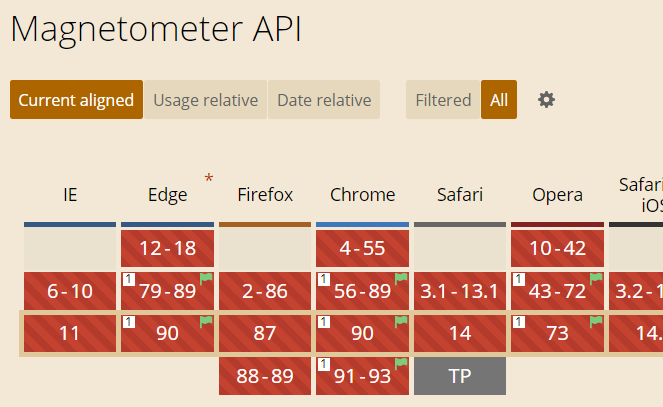
\includegraphics[width=\textwidth]{images/magneto2.png}}
    \caption{caniuse.com - Magnetometer API}
\end{figure}

\subsection{Workspace Management}
\paragraph{Making a Consistent Server and Covering Failure Cases}
As the workspace management handles storage of user data, it acts as a bridge between the client and the model management. Thus the validity of these data is a very crucial part of the work. Although the client prevents most of the invalid requests, such invalid requests could be handcrafted and sent to the server or the client itself could possibly generate an invalid data by an error so each request needed to be validated. Finding the error cases and handling them generated a lot of work, because finding the not so obvious error cases needed a general analysis of the action caused by the request on the server and possibly on the model management.
\paragraph{Performance-Space Trade-Off Decisions}
TBD
\subsection{Model Management}
\subsection{Auth}
